\documentclass[a4paper,11pt,oneside,openany]{report}
%
%%%%%%%%%%%%% DO NOT DELETE BELOW %%%%%%%%%%%%%%%%
\makeatletter
\def\clap#1{\hbox to 0pt{\hss #1\hss}}%
\def\ligne#1{%
\hbox to \hsize{%
\vbox{\centering #1}}}%
\def\haut#1#2#3{%
\hbox to \hsize{%
\rlap{\vtop{\raggedright #1}}%
\hss
\clap{\vtop{\centering #2}}%
\hss
\llap{\vtop{\raggedleft #3}}}}%
\def\bas#1#2#3{%
\hbox to \hsize{%
\rlap{\vbox{\raggedright #1}}%
\hss
\clap{\vbox{\centering #2}}%
\hss
\llap{\vbox{\raggedleft #3}}}}%
\def\svb#1#2{%
  \hbox to \hsize{%
    \hbox to 0.5\hsize{\hfil #1:}%
    \hbox to 0.4\hsize{~#2 \hfil}}}%
\def\maketitle{%
\thispagestyle{empty}\vbox to \vsize{%
\haut{}{\LARGE \textbf{\@thesistype}}{}
\vfill
\ligne{\Huge \@title}
\vspace{1cm}
\ligne{\LARGE \@author}
\bigskip
\ligne{\Large \@studentid}
\vfill
\haut{}{\Large \@affiliation}{}
\vfill
\ligne{\Large \@supervisor}
\ifx\@dsupervisor\@empty\else
  \medskip \svb{\Large \@dsupervisorname}{\Large \@dsupervisor}
\fi
\vfill
\bas{}{\large \@date}{}
}%
\cleardoublepage
}
\def\date#1{\def\@date{#1}}
\def\author#1{\def\@author{#1}}
\def\studentid#1{\def\@studentid{#1}}
\def\title#1{\def\@title{#1}}
\def\supervisor#1{\def\@supervisor{#1}}
\def\dsupervisor#1{\def\@dsupervisor{#1}}
\def\supervisorname#1{\def\@supervisorname{#1}}
\def\dsupervisorname#1{\def\@dsupervisorname{#1}}
\def\affiliation#1{\def\@affiliation{#1}}
\def\thesistype#1{\def\@thesistype{#1}}
\title{}
\author{}
\date{}
\supervisor{}
\dsupervisor{}
\supervisorname{}
\dsupervisorname{}
\affiliation{}
\thesistype{}
\makeatother
%
%
%
\pagestyle{plain}
\supervisorname{Supervisor}
\dsupervisorname{Deputy Supervisor}
\renewcommand{\abstractname}{\Large Abstract}
\renewcommand{\bibname}{References}
\usepackage[left=30mm, right=30mm, top=25mm, bottom=25mm]{geometry}
\newcommand{\tabincell}[2]{\begin{tabular}{@{}#1@{}}#2\end{tabular}}
%
%
%%%%%%%%%%%%% DO NOT DELETE ABOVE %%%%%%%%%%%%%%%%
%
%
% User Defined Packages
%
\usepackage{amsmath,amssymb}
\usepackage{courier}
\usepackage{bm}
\usepackage{graphicx}
\usepackage{subfigure}
\usepackage{verbatim}
\usepackage{wrapfig}
\usepackage{ascmac}
\usepackage{myref}
\usepackage[sort]{cite}

% Use these packages to beautify latex template
\usepackage[T1]{fontenc}
\usepackage{charter}
\usepackage[expert]{mathdesign}
\usepackage{booktabs}
\usepackage{ltablex}
\usepackage{siunitx}
\usepackage{threeparttable}

\usepackage{fancyhdr}
\usepackage{exsheets}
\usepackage[framemethod=TikZ]{mdframed}
% for code
\usepackage[utf8]{inputenc}

\usepackage{listings}
\usepackage{color}
\usepackage{booktabs}

\definecolor{codegreen}{rgb}{0,0.6,0}
\definecolor{codegray}{rgb}{0.5,0.5,0.5}
\definecolor{codepurple}{rgb}{0.58,0,0.82}
\definecolor{backcolour}{rgb}{0.95,0.95,0.92}

\lstdefinestyle{mystyle}{
	backgroundcolor=\color{backcolour},   
	commentstyle=\color{codegreen},
	keywordstyle=\color{magenta},
	numberstyle=\tiny\color{codegray},
	stringstyle=\color{codepurple},
	basicstyle=\footnotesize,
	breakatwhitespace=false,         
	breaklines=true,                 
	captionpos=b,                    
	keepspaces=true,                 
	numbers=left,                    
	numbersep=5pt,                  
	showspaces=false,                
	showstringspaces=false,
	showtabs=false,                  
	tabsize=2
}

\mdfsetup{
	roundcorner=5pt
}

\lstset{style=mystyle}

\newcommand{\resultRelated}[1]{#1}

\fancyhf{}
\fancyhead[L]{\slshape \leftmark}
\fancyfoot[C]{\thepage}
\pagestyle{fancy}
%
%
%%%%%%%%%%%%%%%%%%%%%%%%%%%%%%%%%%%%%%%%%%%%%%%%%%
%
%
\thesistype{Master's Thesis}
%\thesistype{Doctoral Dissertation}
\title{Deep Learning based Semantics Model for Software Defect Prediction}
\author{Jidong Li}
\studentid{17M38124}
\affiliation{
  Graduate Major in Computer Science\\
  School of Computing\\
  Tokyo Institute of Technology
}
\date{January, 2020}
\supervisor{Supervisor: Takashi Kobayashi}
%\dsupervisor{Jiro Kogaku}
%
\begin{document}
%
%
\maketitle
%
%
%
%
\tableofcontents
\listoffigures
\listoftables
%
%
\clearpage
\setcounter{page}{1}
\chapter{Introduction}
\section{Motivation}
Software defect prediction(SDP) is kind of technique for software checking and the debugging. It will cost much for a software maintenance at later period. Since,By using SDP, the developers can focus on the modules that most likely have bug.\\
\\
Recent technique mainly base on machine learning model to predict the whether a file or a bug have bug or not. this method mainly make use of history data, then construct a series of metrics to train the model, so that it can be utilized to predict the buggy of other modules.\\

Since building a effective metric is essential in a machine learning model, many researcher have proposed their concept and idea to construct the metric of SDP model, in the early research, Line Of Code (LOC)\cite{} was employed to measure if file that have bug or not. However, such simple metric ignores the structure of code. Halstead proposed a software complexity metric by counting the occurrence of operator and operand in the source code \cite{}. McCabe also raise concept of cyclomatic complexity that possibility of causing bugs increase as the program becomes more complex\cite{}. CK metrics suit measures the software complexity by considering its inheritance, coupling, and cohesion. MOOD \cite{} metrics are also be proved as effective in SDP. \\

As for machine learning model, many classical machine learning model are adopted for SDP. such as logistics regression (LR), support vector machine (SVM),decision tree (DT), random forest (RF), Adaboost, and naive bayes (NB). Moreover, ensemble learning strategy such as voting, stacking and averaging are perform well in SDP. 

However, traditional machine learning base model may have some problem:
\begin{itemize}
    \item Need to construct metric manually.
    \item Do not consider the semantics of code.
\end{itemize}

Traditional machine learning model need to extract features manually to construct a machine learning model. Thereby, the quality of feature is directly impact the performance of machine learning model. Besides, traditional metrics did not consider the semantics of programs. Take Figure 1.1 as example, \texttt{foo()} function and \texttt{bar()} fucntion has the same of count of line of code. When we select \texttt{add()} and \texttt{remove()} as the information node of these two code snippets, we will generate [\texttt{add(0)},\texttt{remove(0)},\texttt{remove(0)},\texttt{add(0)}] and [\texttt{add(0)},\texttt{remove(0)},\texttt{add(0)},
\texttt{remove(0)}] for \texttt{foo()} and \texttt{bar()},respectively. However, \texttt{foo()} will occur exception. Traditional metrics can not identify such feature, so called semantics features. To solve this problem. Wong et.al \cite{} extract abstract syntax tree (AST) and select specific node from AST to present the code semantics, then they leverage word embedding technique to embed word into vectors and Finally employed deep belief network (DBN) \cite{} to extract feature from the embeded AST nodes and achieved better performance than traditional models. Song et.al also adopted Convolutional Neural Networks (CNN) to extract the features of programs, which also perform better than traditional machine learning model. Tree-base LSTM was employed to solve different level semantics of programs.\\

\begin{figure}
    \centering
    \subfigure[]{
    \begin{minipage}[t]{0.48\linewidth}
    \centering
    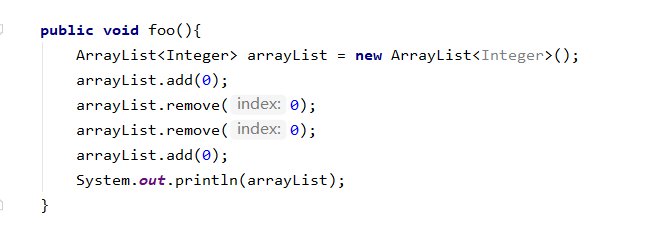
\includegraphics[width=3in]{pic/foo.png}
    \end{minipage}
    }
    \subfigure[]{
    \begin{minipage}[t]{0.48\linewidth}
    \centering
    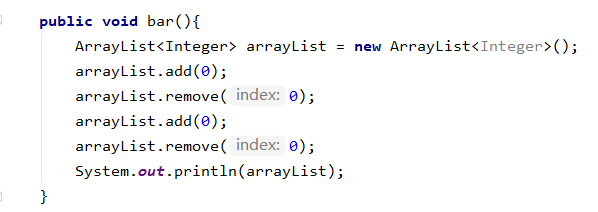
\includegraphics[width=3in]{pic/bar.png}
    \end{minipage}
    }
    \caption{a motivation example}
\end{figure}

Undoubly, such existing deep learning model can effective improve the performance of SDP, however, they still have some problems 
\begin{itemize}
    \item Limited by training data, the token may not be trained sufficiently.
    \item Not be able to learn identical tokens semantics in different context
\end{itemize}

Limited by existing public defect dataset, the number of instance in the largest project is no more than 2000, thereby tokens may not be trained sufficiently in token embedding phrase. Besides, it can also llanguage model. Different from \textit{Word2vec} model, the \textit{BERT} model can learn the ead to overfiting problem when deep learning model constructed with large count parameter. To solve this problem, we proposed data augmentaion strategy to generate more data for training. To ensure that token can be well-trained, we pretrain large Java source code using  \textit{BERT} semantics of identical token under different semantics. \\

On the one hand, tokens in training data not appeared in test data which will impact the performance of model.On the other hand, existing researches mainly select specific nodes from ASTs tree and generate sequence. Though, such kind of approaches can learn the semantics of source code, whereas it ignore large kind node. The result is that vocabulary size become smaller compare with the approach that use all tokens from source code. \\ 

Since attention based LSTM and CNN are show excellent performance in text classification and previous, we make use of both ability to learn the semantics to generate features. BiLSTM can learn context information in a sequence while attention mechnism can foucs the token with important information. CNN can learn the local information of sequence. Both two approach are widely applied in academic research and industry.

Base on the problem that given above, we raise several research questions to validate the effectiveness of our model.\\

\textbf{RQ1:Can data augmentation improve the performance of our model?}. To verify our assumption that more data for training can improve the performance, we conducted the experiment by boosting training dataset. 

\textbf{RQ2: Can our model outperform other models including traditional metrics based models and deep learning based models?}. To verify whether our model are better than existing deep learning model, we select to deep learning models, CNN model as baseline to compare with our model. For traditional features base model, we construct two baseline with logistics regression as traditional model.

\textbf{RQ3: Is BERT prtreained model Better than Word2vec pretrained model}. We investigate which kind of information are better for SDP.

\textbf{RQ4: Which data preprocessing method is better for Software defect prediction?}. Since mainly researches parse source code into ASTs while another is make use all the tokens. We compare both two preprocessing method to investigate which form is better for SDP.

The rest part of this paper is follows. Chapter 2 introduce the relevant researches and background; chapter 3 introduces the details of proposed model; chapter 4 ilustrate how we design the experiments for research questions; chapter 5 is the results of our experiments; chapter 6 is discussion of our results; chapter 7 is the conclusion of our experiments.






\chapter{Background \& Related Works}
\section{Software Defect Prediction}
% 此处需要一张图
In this section, we introduce the related work of software defect prediction. Since machine learning based approach many contain two phase, one is defect metric, another is machine learning model. Figure 4 show the general framework of machine learning base model. 
\begin{figure}
    \centering
    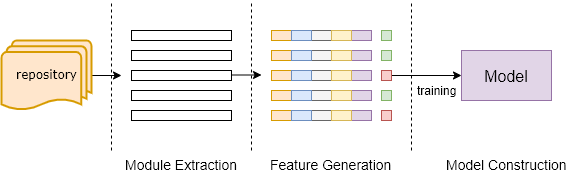
\includegraphics[width=12cm,height=4cm]{pic/defect_overview.png}
    \caption{general framework of machine learning based model}
    \label{fig:my_label}
\end{figure}
\subsubsection{Module Extraction}
To construct a SDP model, the first step we need to extract modules from project, the level can be module, file or function module. Using defect tracking system to label whether each module has bug or not.
\subsubsection{Feature Generation}
The next step is feature generation; after we obtain modules, we need to generate features for each module, their two primary methods to generate feature, one is to apply designed metric to create the feature, another is using deep learning automatically make the feature.
\subsubsection{Model Construction}
After we obtain features and labels of project, i.e dataset, we need to preprocess the dataset so that it can fit the model we selected. Generally, The main problems in the data preprocessing process are data imbalance, data loss and data normalization. Then adopt suitable classification algorithm train a model. Finally, apply the trained model to make other data pretrained 
\subsection{Software Defect Metrics}
There are many forms of metric construction approach, mainly can be divided into three forms of pattern: code-based approach and process-based approach.

\subsubsection{Code-based Approach}
In the early age, Akiyama \cite{} employed \textit{line of code} as metric for SDP. The more code in a file or module, The more likely a file or module have bugs. However, LOC is simple and not enough to indicate the complexity of program. Thereby, in later research, Halstead and MaCabe metric consider the cyclomatic complexity of programs. Halstead metric \cite{} believe that the count of  operand and operator impact program reading speed for reader. The more difficult to read a program, the more possible it contains bug. McCabe metric mainly foucs on control flow of program, if a control flow has higher in this approach. The complexity of the control flow in a program decide whether it has bug or not. However, and the formula is $v(G)=e-n+2$, where $e$ is amount of edge, $n$ is amount of node. In addition, it can calculate the essential complexity and design complexity. With prevalence of OOP, Many researchers begin to design metric for OOP. One of most important metric is CK metric proposed by Chidamber and Kemerer \cite{}. CK metric consider the important of the most coupling, inheritance and cohesion of programs. 

\subsubsection{Process-based Approach}
Software defect are not only associate with code itself, but also associate with external factor. developers' experience and churn of code may result defect problem in software development. 


\section{Deep learning based Software defect Prediction}
With the popularity of NLP development, many researcher begin to apply NLP technique in SDP domain.The advantages of deep learning approach can learn the semantics and syntax of program, which is ignored by traditional model. Such kind of approach show excellent performance compare with traditional machine learning approach.\\

Wang \cite{} extract specific node from AST which was extracted from source code. Then convert these nodes into sequence as input of DBN to generate vector to present semantics of program. After that, they built classification model to by using both defect label and the generated features. The performance of this approach are 14.2\% and 8.9\% higher in F-measurement in terms of WPDP and CPDP,respectively.\\

Encouraged by Wang's approach, Li \cite{} utilize Convolutional neural network to construct the SDP model. They learn from wang's approach, generated semantic featrues by extracting AST nodes from source code. Then the features will be an input of convolutional nerual network. The result show that this approach improved F1 score compared with Wang's.\\

However, such approaches did not consider the level of semantics of program, Dam's el.al \cite{} proposed tree-based LSTM to learn different level semantics of program. They convert different level of node of AST into vector and define a loss function to train node vector to generate vector of AST. Using the AST vector to train SDP model. This approach achieved higher score than existing method in recall.\\

However, when constructing a deep learning model, embedding is necessary for downstream task. The general process is pad the sequence into fixed length. However, if long sequence with more information is condensed into fixed length, it will lose part of information. Thereby, Fan et.al \cite{} propose \textit{BiLSTM}+\textit{attention} method to solve the problem. They first apply \textit{BiLSTM} to extract the semantics feature, then use \textit{attention} to calculate the weight of hidden state generated by \textit{BiLSTM}. The model outperform  state-of-the-art model 14\% and 7\% in F-measure and AUC sorce, respectively. \\

The model that mentioned above have similar problem, i.e without pretrained token vector. Since the defect datasets are small, tokens may not be well-trained and will impact the performance of downstream layer. Thereby, Liang el.al \cite{} pretrained large tokens vector to alleviate this problem. And their proposed model outperform other model both on within-project defect prediction and cross-project defect prediction. \\

\section{Word Emebedding}
In NLP domain, word embedding is based process for downstream task. Since present token through one hot vector may spend large strage, thereby, there are many researches are manage to condense one hot vector into dense vector and present its semantics simulaseously. In this section, we introduce some typical and classic method to embed word.\\

\textbf{Word2Vec}\cite{}, This is typical method that transfer token into vector to present its semantics. In \textit{Word2Vec} model, it is kind of supervisor learning and has two form of model. one is \textbf{skip-gram} and another is \textbf{Continuous-Bag-Of-Word} (CBOW). Skip-gram model is to predict the context tokens when given the center word. and \textbf{CBOW} is the model to predict center token given context. \textit{Word2Vec} is widely apply in NLP task. The aim of \textit{Word2Vec} is to train a word vector that can suit multi task of NLP. However, \textit{Word2Vec} can not handle the problems that tokens in different context present different semantics. \\

\textbf{EMLO} \cite{}. To handle this the problem existed in \textit{Word2Vec}. \textit{EMLO} apply \textbf{BiLSTM} to train a language model. Since it consider double direction of context, it can learn the semantics for identical tokens in different context. 

\textbf{GPT} \cite{}. \textit{GPT} construct from \textit{Transformer} \cite{}. Since \textit{Transformer} can learn the longer distance since that can learn distance context information. Compare with \textit{ELMO}, \textit{GPT} leverage the ability of \textit{Transformer}, can learn longer distance semantics features and it outperform \textit{EMLO} compare with other downstream NLP task.

\textbf{BERT}. \textit{BERT} was proposed by \textit{Google}. \textit{GPT} can only learn one side semantics features. \textit{ELMO} just concatenate bi-direction features generated by \textit{BiLSTM}.  \textit{BERT}\cite{} apply bidirectional \textit{transformer} that truely learn bidirectional context information. In our proposed method, we apply the pretrained \textit{BERT} by using fine tuning to extract the feature. 

\chapter{Methodology}

In this section we introduce our proposed method for SDP, Figure 3.1 is the overview of our method. we separate our method into 6 part. 

\begin{figure}
    \centering
    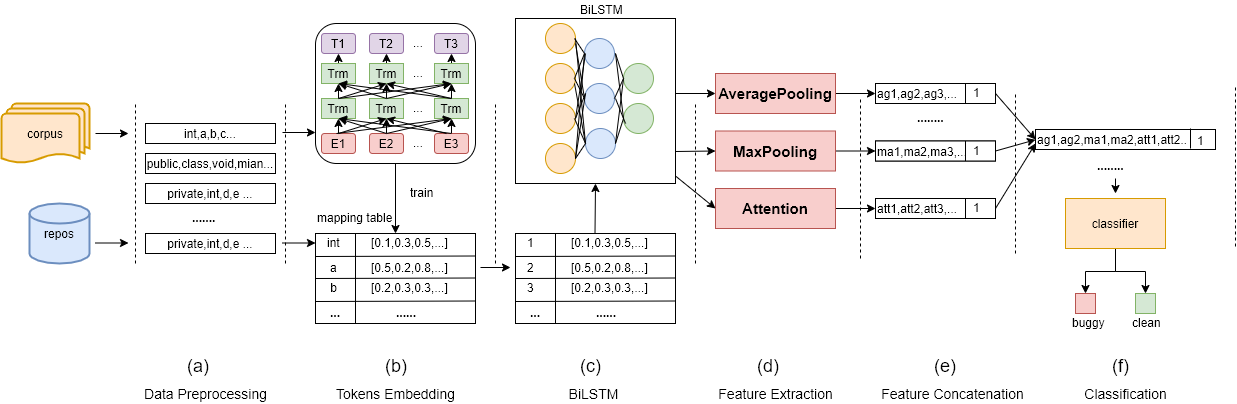
\includegraphics[width=\textwidth,height=0.2\textheight]{pic/model_overview.png}
    \caption{model overview}
    \label{fig:my_label}
\end{figure}

% proprocessing for both dataset and corpus
\section{Data Preprocessing}
In this section, we preprocess our dataset and corpus that fit training, we need to process data and corpus to fit our model. To extract the semantics feature of a program, many research use ASTs (Abstract Synatx Trees) \cite{}to present the semantics of files. However, they just select some forms of nodes from ASTs then concatenate with them, which destroyed the order if original program. Besides, since context information not only hidden in single token, but decided by sequence of tokens. Based on these problem, we directly tokenize Java files. The step can be describled as follow:
%这个地方说明有待加强
\begin{itemize}
    \item Comment removal.We remove all blank lines and comments.
    \item Sequence generation. we directly tokenize all the data to generate the sequence. for each files
    \item We filter out all punctuation and \textbf{string} since we believe it contain less information.
    \item Vocabulary building. We merge all sequence in a project, then count each token's frequency, finally rank each token according to its frequency. We also replace those token whose frequency are lower than our setting with "\textit{unk}". Finally, we padding each sequence wit fixed length.
\end{itemize}

during the processing, we remove all the tokens that has useless information. such as the \texttt{import},\texttt{package} tokens.
% 这个地方图片补充(四张不同的情景图)
% need to explain why 
\subsection{Data Augmentation}
In our dataset, the amount of instance of most projects is no more than 1,000, previous research many focus on data imbalance. However, the entire dataset are still not enough. On the other hand, deep learning method need large volume dataset to train effective model, otherwise, it would be overfitting and is not convincing. Thereby, to construct well-trained data, we learn from method proposed by Li \cite{} to generate specific volume data we need. we generate sequences from one sequence by using following four strategies:
\begin{itemize}
    \item \textbf{Similiar Tokens Replace}. We randomly replace similar tokens for software defect prediction with large corpus 
    \item \textbf{Randomly Insert}. We randomly insert several kinds of tokens into original sequence.
    \item \textbf{Randomly Swap}. We randomly swap two tokens in a sequence.
    \item \textbf{Randomly Delete}. We randomly delete tokens in sequence. 
\end{itemize}

% 这个地方待补充(图和说明)
\section{Token Embedding}
In deep learning process, word embedding is necessary stage for downstream task such as text classification, question answering and machine translation. It is also necessary to make token embedding for our model to yeild the suitable data for training. Thereby, we need to embedding our data to generate model. \\
\textbf{TODO}

\section{Feature Extraction}
\textbf{TODO}
\section{Feature Concatenation}
\textbf{TODO}
\section{Classification}
\textbf{TODO}
\chapter{Experimental Setup}
To answers the research questions that we rasied in chapter 1, we designed the relevant experiments to evaluate our assumption. This most experiments was conducted on our personal laptop. We conduct BERT training with 4 NVIDIA RTX 2080Ti. Here we illustrate how we design the exeriments for each reserach question.

\section{Dataset}
To evaluate our model and other baselines, we decide to adopt  PROMISE dataset. However, since it can not be access now, we use a website called way back machine to visited their history website, and then downloaded the defect dataset, base on each project name and its version, we found its source code. We dropped the file that can not be found base on the file name and path from defect data. The Table 3.1 shows the overveiw of dataset. And description of the data shown in Table 3.2

\begin{table}[h]
    \centering
    \begin{tabular}{c|c|c|c|c}
    \toprule[2pt]
        Project &  Verison & Average & Average(processed) & Defect rate \\
    \toprule[1pt]
        ant &  1.3 \sim 1.7 & 338 & 307 & 0.23 \\
        camel &  1.2, 1.4, 1.6 & 815 & 367 & 0.45 \\
        ivy &  1.1, 1.4 & 176 & 151 & 0.32 \\
        jedit &  3.2.1 4.1 \sim 4.3 & 360 & 325 & 0.17 \\
        lucene &  2.2, 2.4 & 293 & 265 & 0.62 \\
        poi &  1.5, 2.0, 2.5 & 312 & 279 & 0.50 \\
        synapse & 1.1, 1.2 & 239 & 212 & 0.33 \\
        velocity &  1.4.1, 1.6.1 & 213 & 182 & 0.59 \\
        xalan &  2.4 \sim 2.7 & 830 & 739 & 0.58 \\
        xerces &  1.2.0, 1.3.0, 1.4.4 & 410 & 224 & 0.36 \\

    \toprule[2pt]
    \end{tabular}
    \caption{Dataset Overview}
    \label{tab:my_label}
\end{table}

\begin{table}[h]
    \centering
    \begin{tabular}{c|c}
    \toprule[2pt]
        Columns & Description \\
    \toprule[1pt]
        \textit{LOC} & The number of methods in the class \\
        \textit{DIT} & The position of the class in the inheritance tree \\
        \textit{NOC} & The number of immediate descendants of the class\\
        \textit{CBO} & \tabincell{c}{The value increases when the methods of \\ one class access services of another} \\
        \textit{RFC} & \tabincell{c}{Number of methods invoked in response \\ to a message to the object} \\
        \textit{LCOM} & \tabincell{c}{Number of pairs of methods that do not \\ share a reference to an instance variable} \\
        \textit{LOCM3} & \tabincell{c}{If \textit{m,a} are the number of methods,attributes in a class number and \\ is the number of methods accessing an attribute, then locm3=} \\
        \textit{NPM} & The number of all the methods in a class that are declared as public. \\
        \textit{DAM} & \tabincell{c}{Ratio of the number of private (proteced) \\ attributes to the tatal number of attributes.} \\
        \textit{MOA} & \tabincell{c}{The number of data declarations (class fields) \\ whose types are user defined classes.} \\
        \textit{MFA} & \tabincell{c}{Number of methods inherited by a class plus \\ number of methods accessible by member methods of the class.} \\
        \textit{CAM} & \tabincell{c}{Summation of number of different types of \\ method parameters in every method divided by a multiplication of number \\ of different method parameter types in whole class and number of methods} \\
        \textit{IC} & The number of parent classes to which a given class is coupled. \\
        \textit{CBM} & \tabincell{c}{Total number of new/redefined methods to \\ which all the inherited methods are copuled} \\
        \textit{AMC} & The number of JAVA byte codes. \\
        \textit{Ca} & How many other classes use the specific class. \\
        \textit{Ce} & \tabincell{c}{Maximum McCabe's Cyclomatic Complexity \\ values of methods in the same class.} \\
        \textit{Max(CC)} & \tabincell{c}{Maximum McCabe's Cyclomatic Complextity \\ values of methods in the same class.} \\
        \textit{Avg(CC)} & \tabincell{c}{Average McCabe's Cyclomatic Complextity \\ values of methods in the same class.} \\
        \textit{LOC} & Measures the volume of code. \\
    \toprule[2pt]
    \end{tabular}
    \caption{Dataset Overview}
    \label{tab:my_label}
\end{table}

\section{Corpus Pretraining}
To evaluate our model with other deep learning baselines, it is necessary to pretrain a language model for those deep learning model. On the other hand, Since there no pretrained model for source code, especially Java code. Thereby, we pretrained mini version of BERT to statisfy our requirement. 

\subsection{Corpus}
To train a language model, we adopt the part of \textbf{BigCode} \cite{allamanis2018survey}, to genereated the corpus we need. Here is description of the our processed corpus.

\begin{table}[]
    \centering
    \begin{tabular}{c|c|c|c}
        \toprule[2pt]
        \textbf{Number of Line} & \textbf{Total Tokens} & \textbf{Vocabulary Size}  & \textbf{Average Sequence Length}\\
        \toprule[1pt]
        306,522 & 84,955,239 & 2,047,760 & 277 \\
        \toprule[2pt]
    \end{tabular}
    \caption{description of preprocessed corpus}
    \label{tab:my_label}
\end{table}

\subsection{Word2vec}
\textit{Word2vec} is one of most frequently used model in NLP domain. Since many research about source code embedding via using \textit{Word2vec} model, our deep learning based model will adopt the tokens vector table that generated by \textit{Word2vec} model, we use gensim \footnote{https://radimrehurek.com/gensim/}, an open source package including \textit{Word2vec} model. Talbe 4.4 show the trianing settings of Word2vec model.

\begin{table}[h]
    \centering
    \begin{tabular}{c|c|c|c}
        \toprule[2pt]
        Dim Size & Window & min\_count & epochs \\
        \toprule[1pt]
        300 & 5 & 5 & 15 \\
        \toprule[2pt]
    \end{tabular}
    \caption{Word2vec Pretraining Settings}
    \label{tab:my_label}
\end{table}


\subsection{BERT}
Since there no source code \textit{BERT} pretrained model aviliable, we pretrained small bert model for our experiments, Table 4.5 show the settings for our \textit{BERT} pretraining. 
\begin{table}[h]
    \centering
    \begin{tabular}{c|c|c|c}
    \toprule[2pt]
        Total Parameter & hidden layer & batch size & epoch \\
    \toprule[1pt]
         264,241,330 & 64 & 8 & 2 \\
    \toprule[2pt]
    \end{tabular}
    \caption{BERT Pretraining Settings}
    \label{tab:my_label}
\end{table}
Due to the limitation of time, the training configuration we select meet our training requirement. We open source tools \textit{BERT-pytorch} \footnote{https://github.com/codertimo/BERT-pytorch} to complete the pretraining task. We firstly construct \textit{BERT} style vocabulary and then use the vocabulary train our model. The training time took one day. 

\section{Evaluatation Metrics}

To evaluate the abality of defect prediction for SDP model, we adopt three metrics to measure their capability:
%Unclear
\begin{itemize}
    \item \textbf{Precision} measure the ability that how well a model that can correct defect instance in all predicted defect label.
    \item \textbf{Recall} measure the how well that defect instance can be predicted successfully.
    \item \textbf{F1} balances the \textbf{Precision} and \textbf{Recall} when we need to take both into account.
\end{itemize}
Below description are the equations of there metrics.
\begin{equation}
    \textbf{Precision}=\frac{TP}{TP+FP}
\end{equation}

\begin{equation}
    \textbf{Recall}=\frac{TP}{TP+FN}
\end{equation}

\begin{equation}
    \textbf{F1}=\frac{2*Precision*Recall}{Precison+Recall}
\end{equation}

where \textit{TP}, \textit{FP} and \textit{FN} are  \textit{True Positive}, \textit{False Positive} and \textit{False Negative}, respectively. \textit{True Positive} is the number of predicted defective example whose true label is defect, \textit{FP} is number of predicted defective example whose true label is clean. \textit{False Negative} is the number of predicted clean example whose true label is defect.

\section{Baseline metrics}
We use two base metrics for experiments for traditional methods. 
\begin{enumerate}
    \item \textbf{Tokens}:We generate this token feature by transforming sequence tokens into sequence of index according to token vocabulary.
    \item \textbf{Stats}:Statistical feature that directly from defect data described in section 4.1.
\end{enumerate}

\section{Baseline Methods}
The following are the baseline methods we selected to compare with our \textit{BERT} based method.

\begin{enumerate}
    \item \textbf{TextCNN}: Deep learning method for text classification. In our experiments, we use three kind of filters whose size are 2,3 and 4, respectively. The number of every filter is 32.
    \item \textbf{BiLSTM+ATT}:Widely applied deep learning method for text classification, we use sentence classification for our experiment.
    \item \textbf{Tokens+LR}: We use \textbf{Tokens} feature to train logistics regression model. 
    \item \textbf{Stats+LR}:We use \textbf{Stats} feature to train logistics model.
\end{enumerate}

\section{Within-Project Defect Prediction}
Within-Project Defect Prediction (WPDP) are the one form of SDP that conducted for individual project. WPDP is general evaluation strategy for many research \cite{}, in our dataset, each project contain several history version. Since WPDP require at least two history version,we filter those projects do not meet this requirement. We trained a model by using previous history versions and evaluate model using the latest version in the project dataset.  For those project with multi-version, we concatenate them into training set. We use the feature generated by our the pretrained model.

\section{Cross-Project Defect Prediction}
In SDP domain, the shortage of defect dataset is key point for the development of research, to relief this problem, Cross-Project Defect Prediction (CPDP) is another form to evaluate SDP model. CPDP train a model using a project dataset and then use the another project to evaluate the performance of the trained model, In our experiments, we have 10 projects, we first concatenate each history version dataset of a project into project dataset, when conducting the CPDP experiments, each project dataset is like to be the target project dataset, similarly, after we generate the project dataset, we concatenate the rest 9 projects dataset as training set for models. For different research question, then for each project, we generated pair dataset.

\section{Parameters Setting}
To investigate the most optimal number of hidden units, we conduct the experiment to find out the most proper number of hidden node for our model,we conduct the experiment to find out the most the most president of our methods. \\
\textbf{TODO}

\section{Experiment for RQ1}
To verify whether data augmentation strategy can improve the performance of data, we adopted our data augmentation strategy to generate more instance for each project. Since our data augmentaion strategy is suitable for small dataset, we conduct WPDP experiment to verify whether our data augmentation can improve the performance of model. On the other hand, to many augmented data may not be able to learn the raw data semantics feature. So we need to find proper augmented times to ensure the maximum performance of models. In this experiment, we select the number range of augmentation are 2,4,8,16,32 and 32. To eliminate those project whose instance's amount are more than 1000 since we believe that data augmentation is more effective on small dataset. In this experiment, we conduct WPDP experiment for our research, since the volume of training data is much larger than that of WPDP.
\section{Experiment for RQ2:Performance comparsion}
To compare with other baseline methods, we conduct the experiment on both WPDP and CPDP we use the F1 score, precision and recall as metrics to measure the performance.
\section{Experiment for RQ3:Embedding comparsion}
To verify which kind of embedding method is effective, we compare with our pretrained mini-version \textit{BERT} model and \textit{Word2vec}, we conduct both WPDP and CPDP for \textbf{TextCNN} and \textbf{BiLSTM+ATT}. 
\section{Experiment for RQ4:Data Preprocessing Method comparsion}
\textbf{TODO}





\input{5.1-results.tex}
\chapter{Discussion}
\textbf{TODO}

\chapter{Conclusion}
\textbf{TODO}
%
%
%
%
\chapter*{Acknowledgment}
\addcontentsline{toc}{chapter}{Acknowledgment}

%
%
%
%
%
\addcontentsline{toc}{chapter}{\bibname}
\bibliographystyle{plain}
\bibliography{./bibtex/cite}
%
%
\end{document}
